\chapter{Implementatie}\label{chap:q2}
In dit hoofdstuk wordt het design van het proof of concept (PoC) die gebruik maakt van smart contracts en blockchain technlogie behandeld. Eerst worden de verschillende actors (gebruikers) gedefineerd waarbij de user stories worden vastgesteld, om te voorzien van de functionele requirements van het PoC.
\par

- quality attributes\newline
- c4.
%specifications for the PoC. Further descriptions of the PoC such as quality attributes and how to set the system of smart contracts up with a blockchain are also given. Thereafter a schematic of the prototypical interactions on the blockchain is shown along with the interactions between the smart contracts. The suggested solution to the described problem uses the decentralised, trust-less and immutable properties of blockchain technology as well as permissioning in the smart contracts. To be noted is, however, that no security or privacy liabilities outside of the blockchain have been resolved with this implementation. Some of the larger off-chain issues are mentioned
%in the discussion.
\newpage

\section{User stories en requirements}
De scope van de implementatie beschreven beperkt zich tot de volgende gebruikers:
verzekeraar, verzekerde en makelaar. Om zo compleet mogelijk alle functionele requirements te noteren is in de onderstaande tabel \ref{fig:userstories} de user stories vanuit de verschillende gebruikers perspectief geschreven. De verschillende gebruikerstypes worden daarna meer in detail gedefinieerd. Er is tijdens het opstellen van de requirements gekozen om alleen het essentiële op te schrijven en deze zoveel mogelijk de versimpelen. Te weten dat, het gebruiksgemak en security eisen van de PoC op een rendabel niveau moeten zijn.

\begin{figure}[h!]
    \begin{center}
        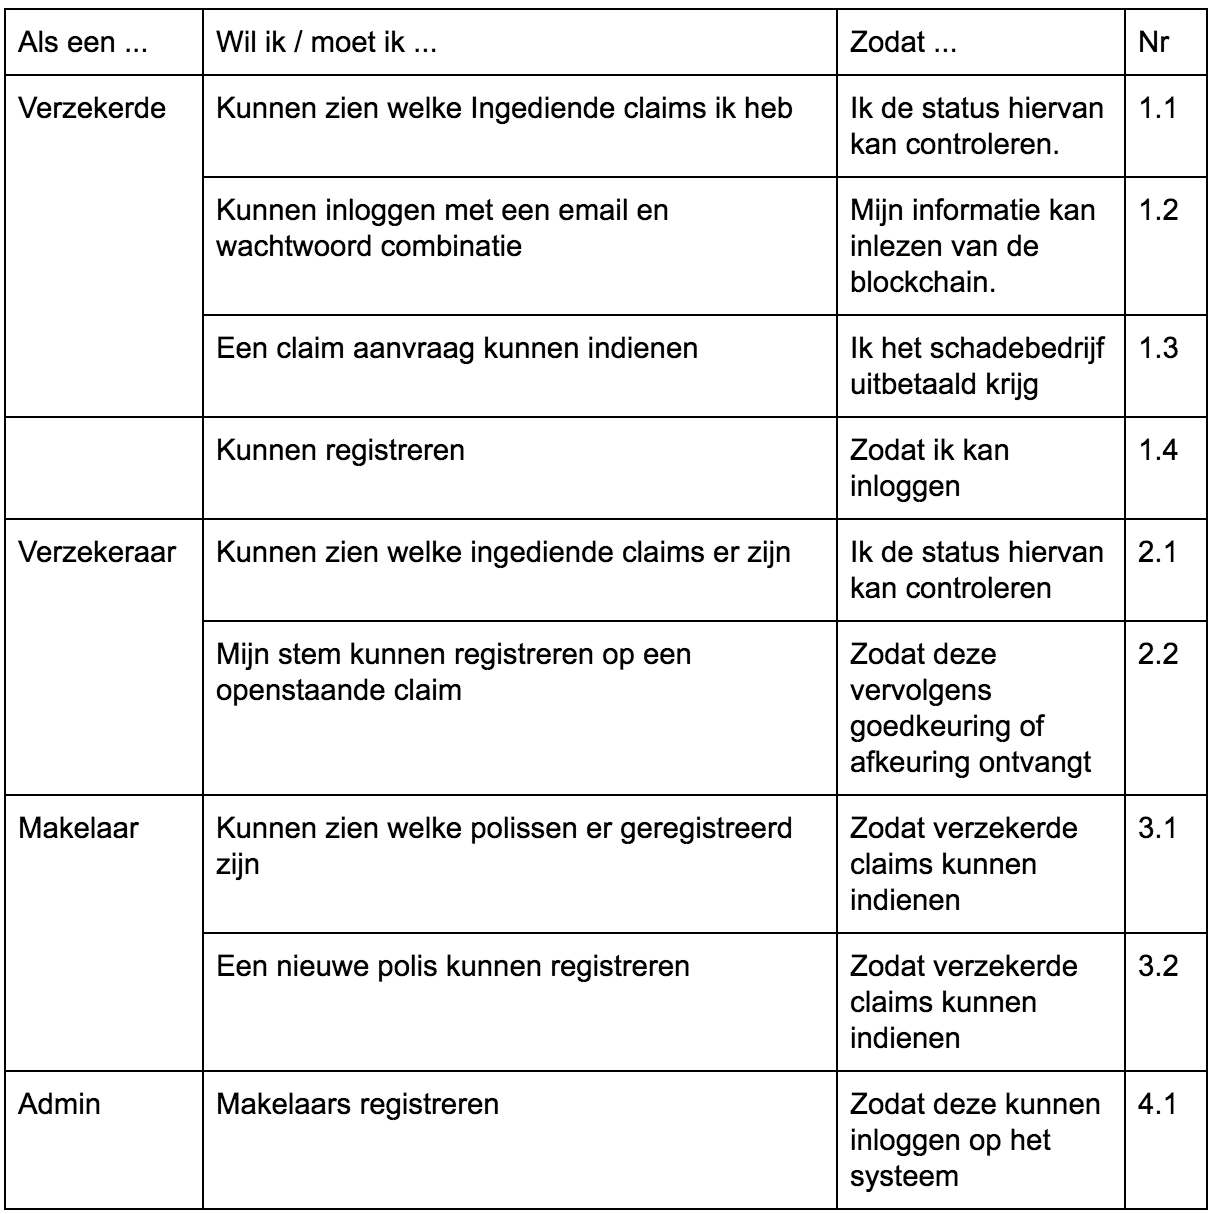
\includegraphics[scale=0.7]{images/userstories}
        \caption{User stories die de functionele requirements defineren en het development van het proof of concept leiden.}
        \label{fig:userstories}
    \end{center}
\end{figure}

\newpage

\begin{figure}[h!]
    \begin{center}
        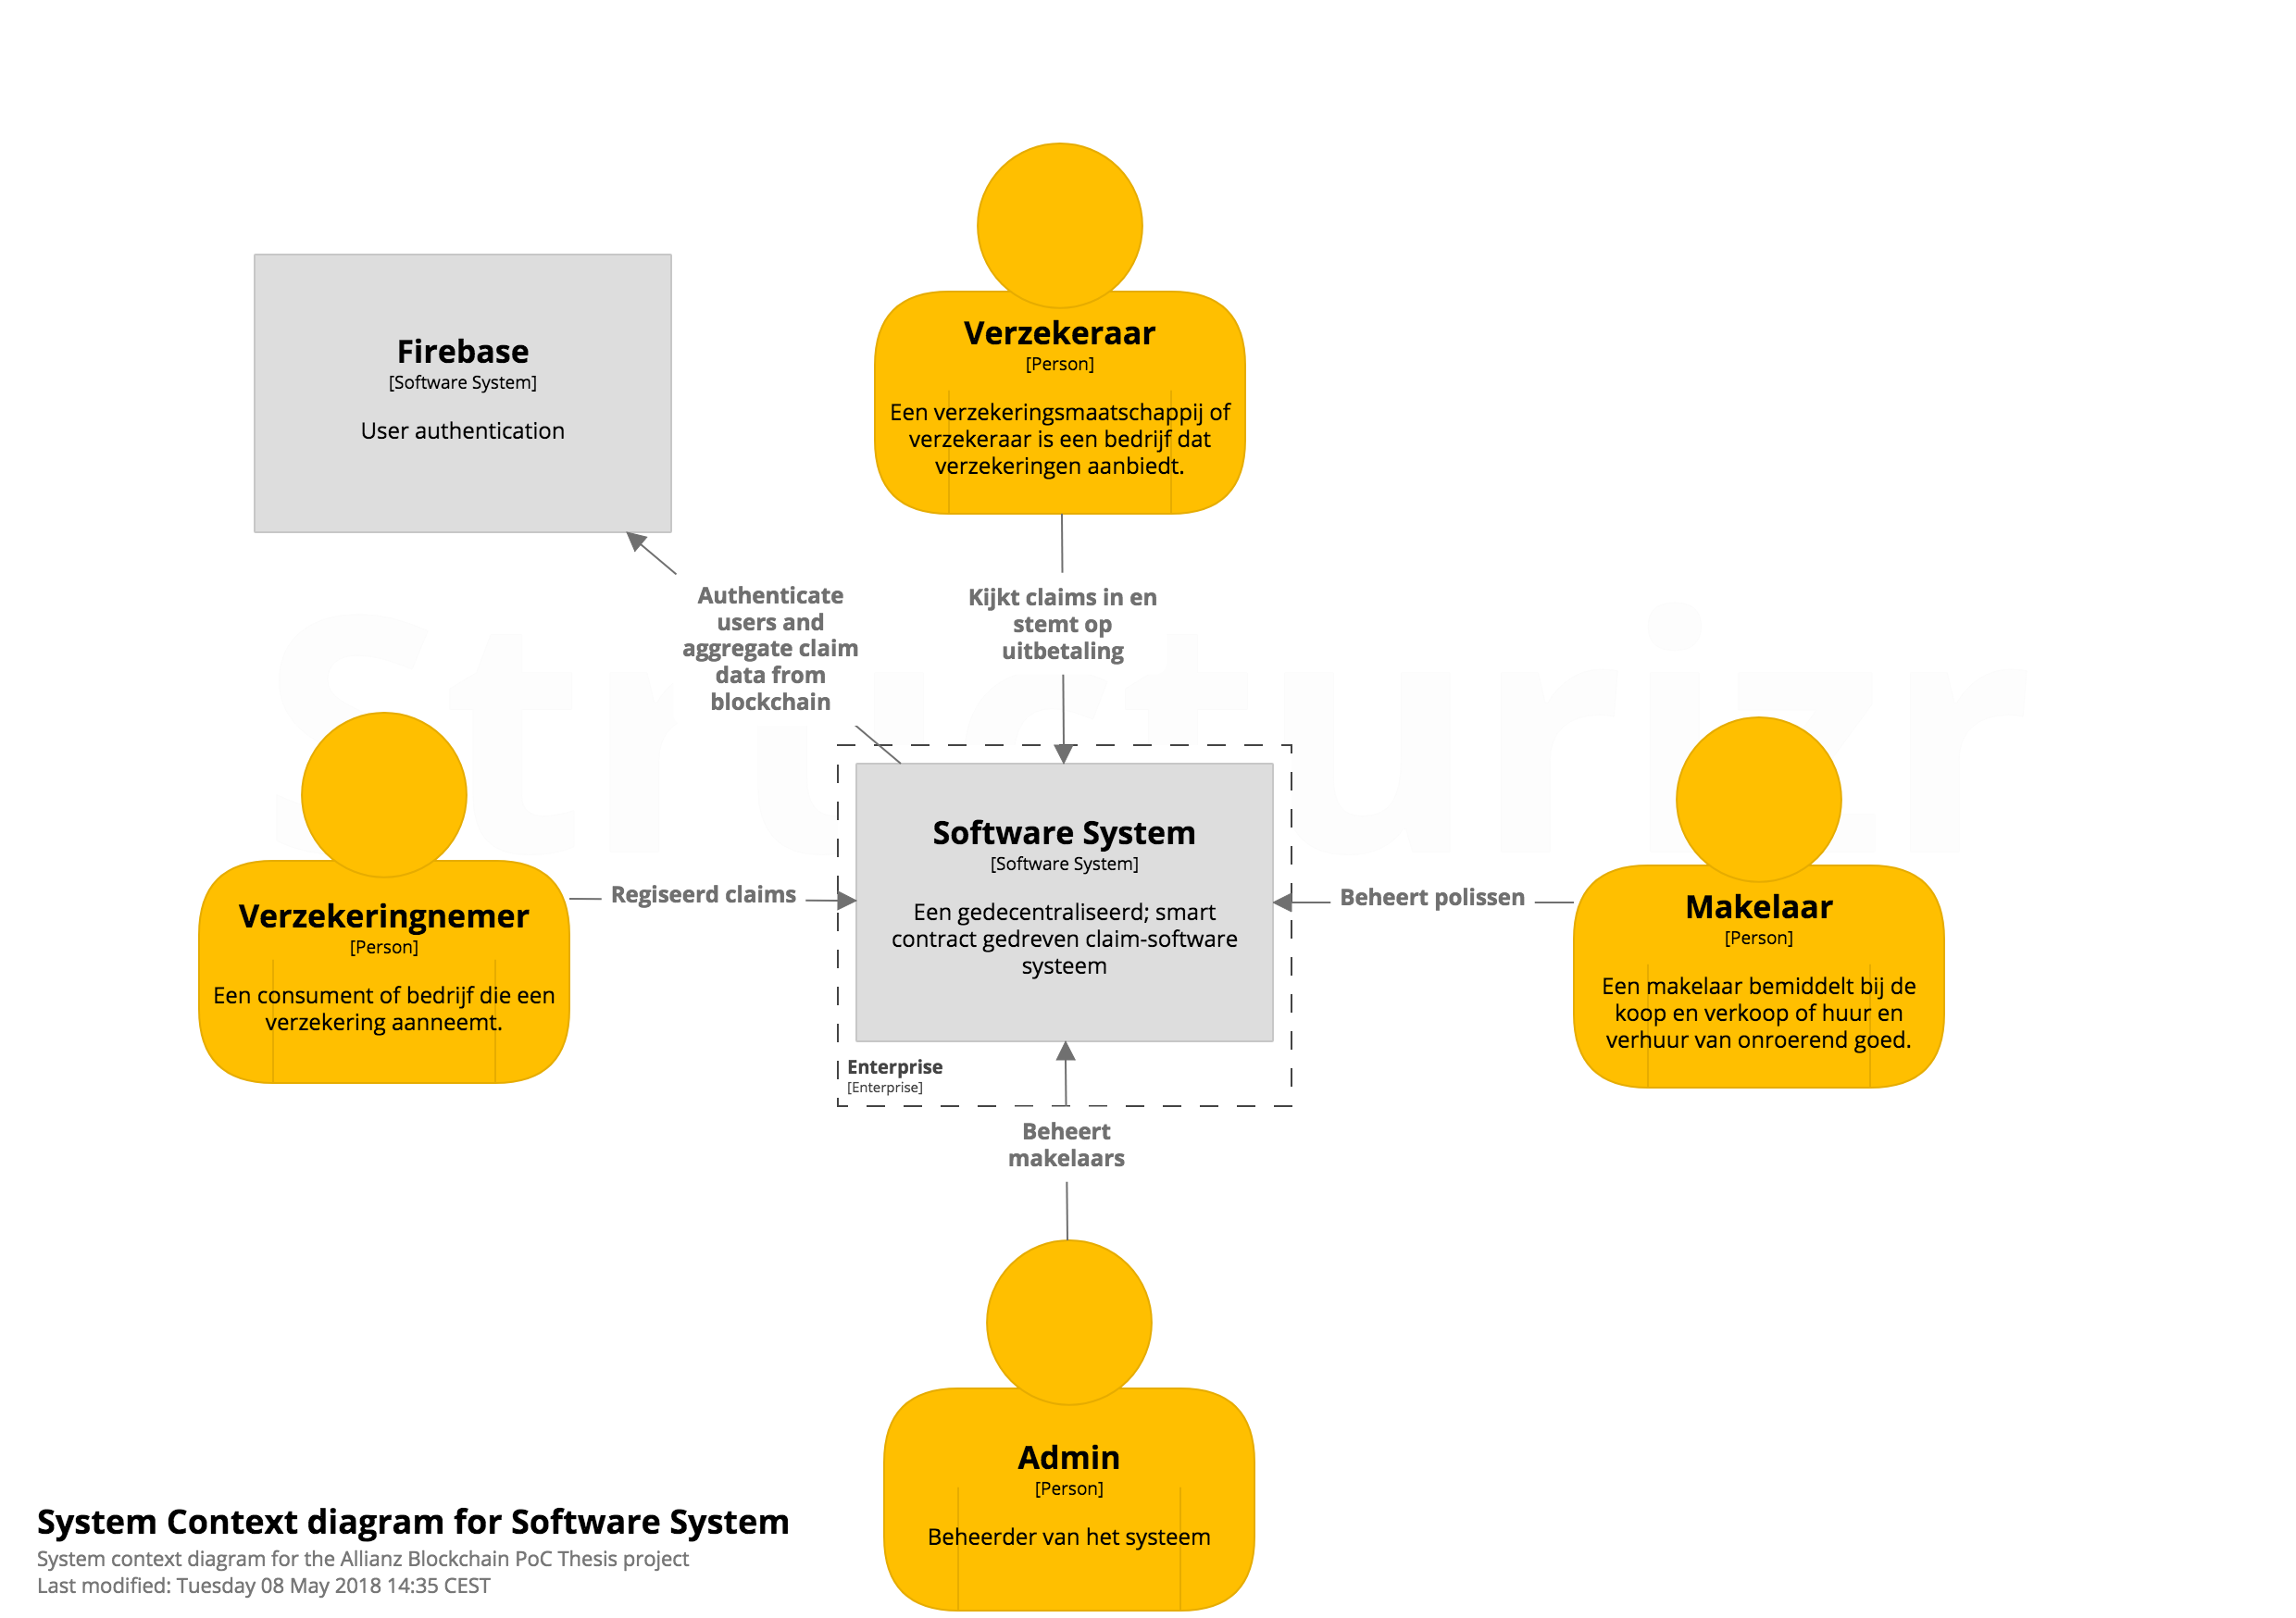
\includegraphics[width=\paperwidth-100]{images/context}
        \caption{C4 - Context.}
        \label{fig:c4Context}
    \end{center}
\end{figure}

Verzekernemers zijn consumenten of bedrijven die een verzekering heeft en met een polisnummer claims kan aanvragen en de status van kan ophalen. De manier waarop gebruikers via de backend interactie hebben met de smart contract in de Ethereum blockchain word getoond in figuur \ref{fig:c4Context}.

\begin{figure}[h!]
    \begin{center}
        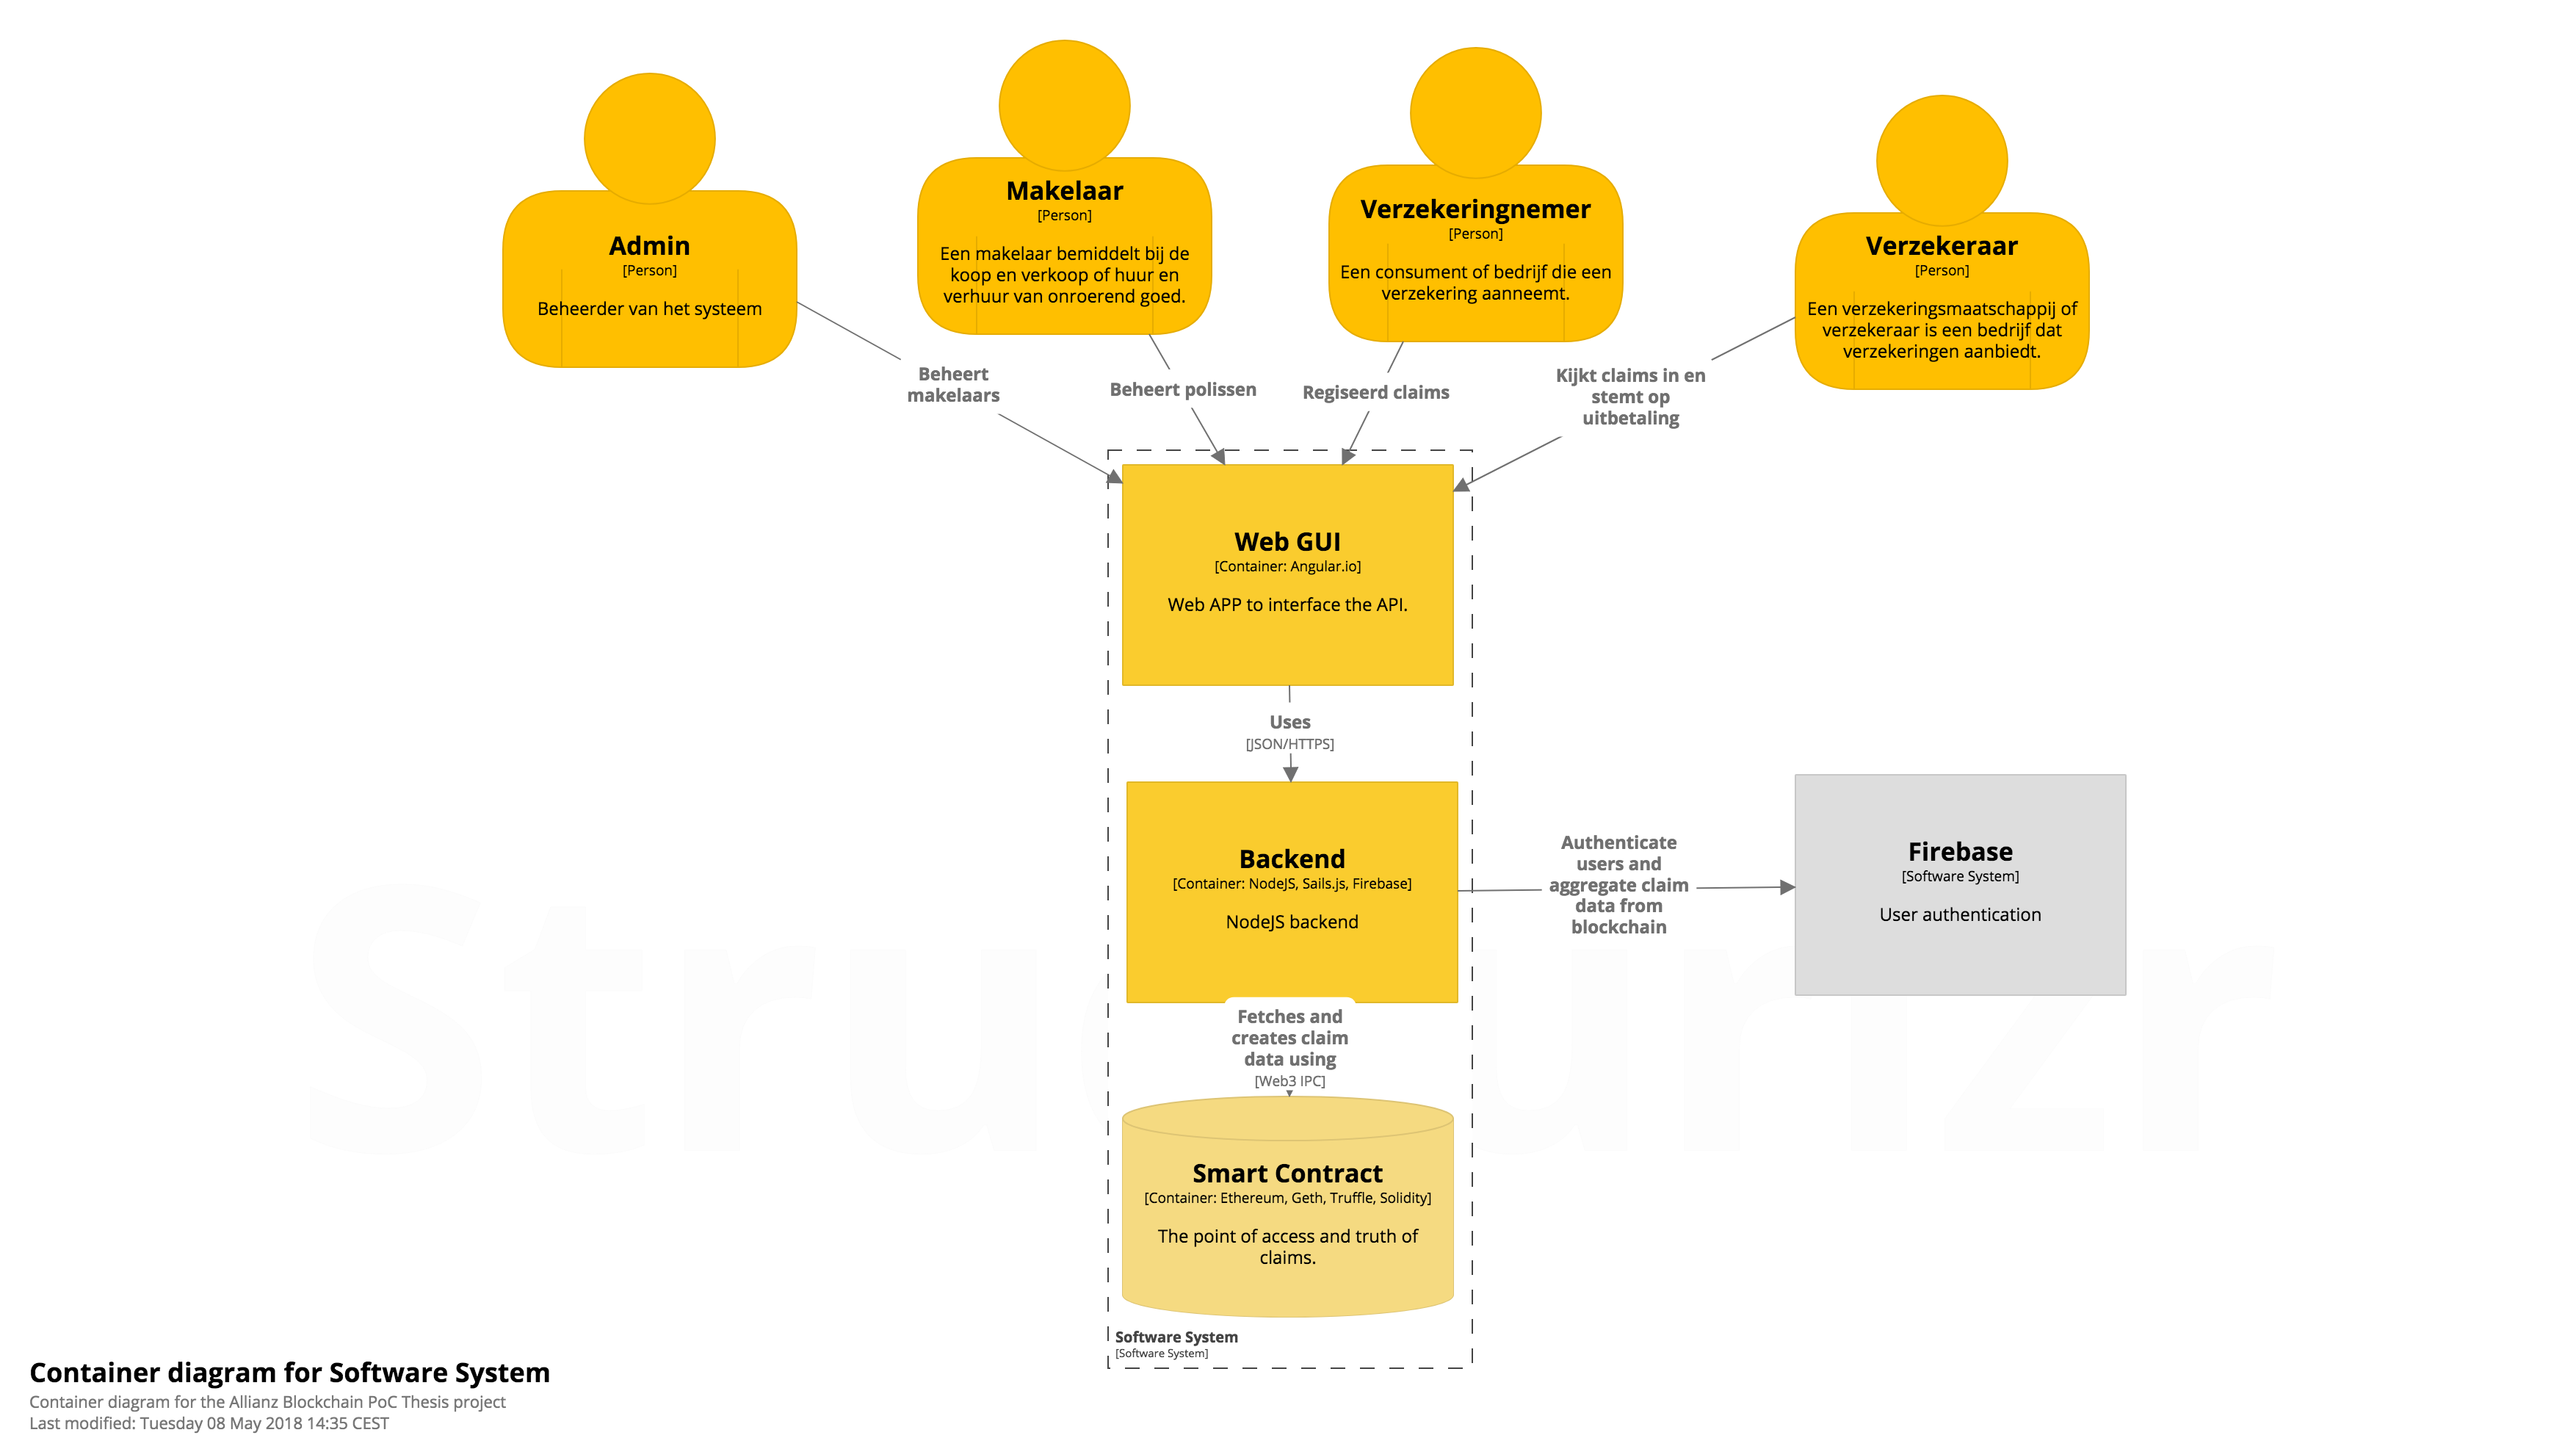
\includegraphics[width=\paperwidth-100]{images/containers}
        \caption{C4 - Containers.}
        \label{fig:c4Containers}
    \end{center}
\end{figure}

\begin{figure}[h!]
    \begin{center}
        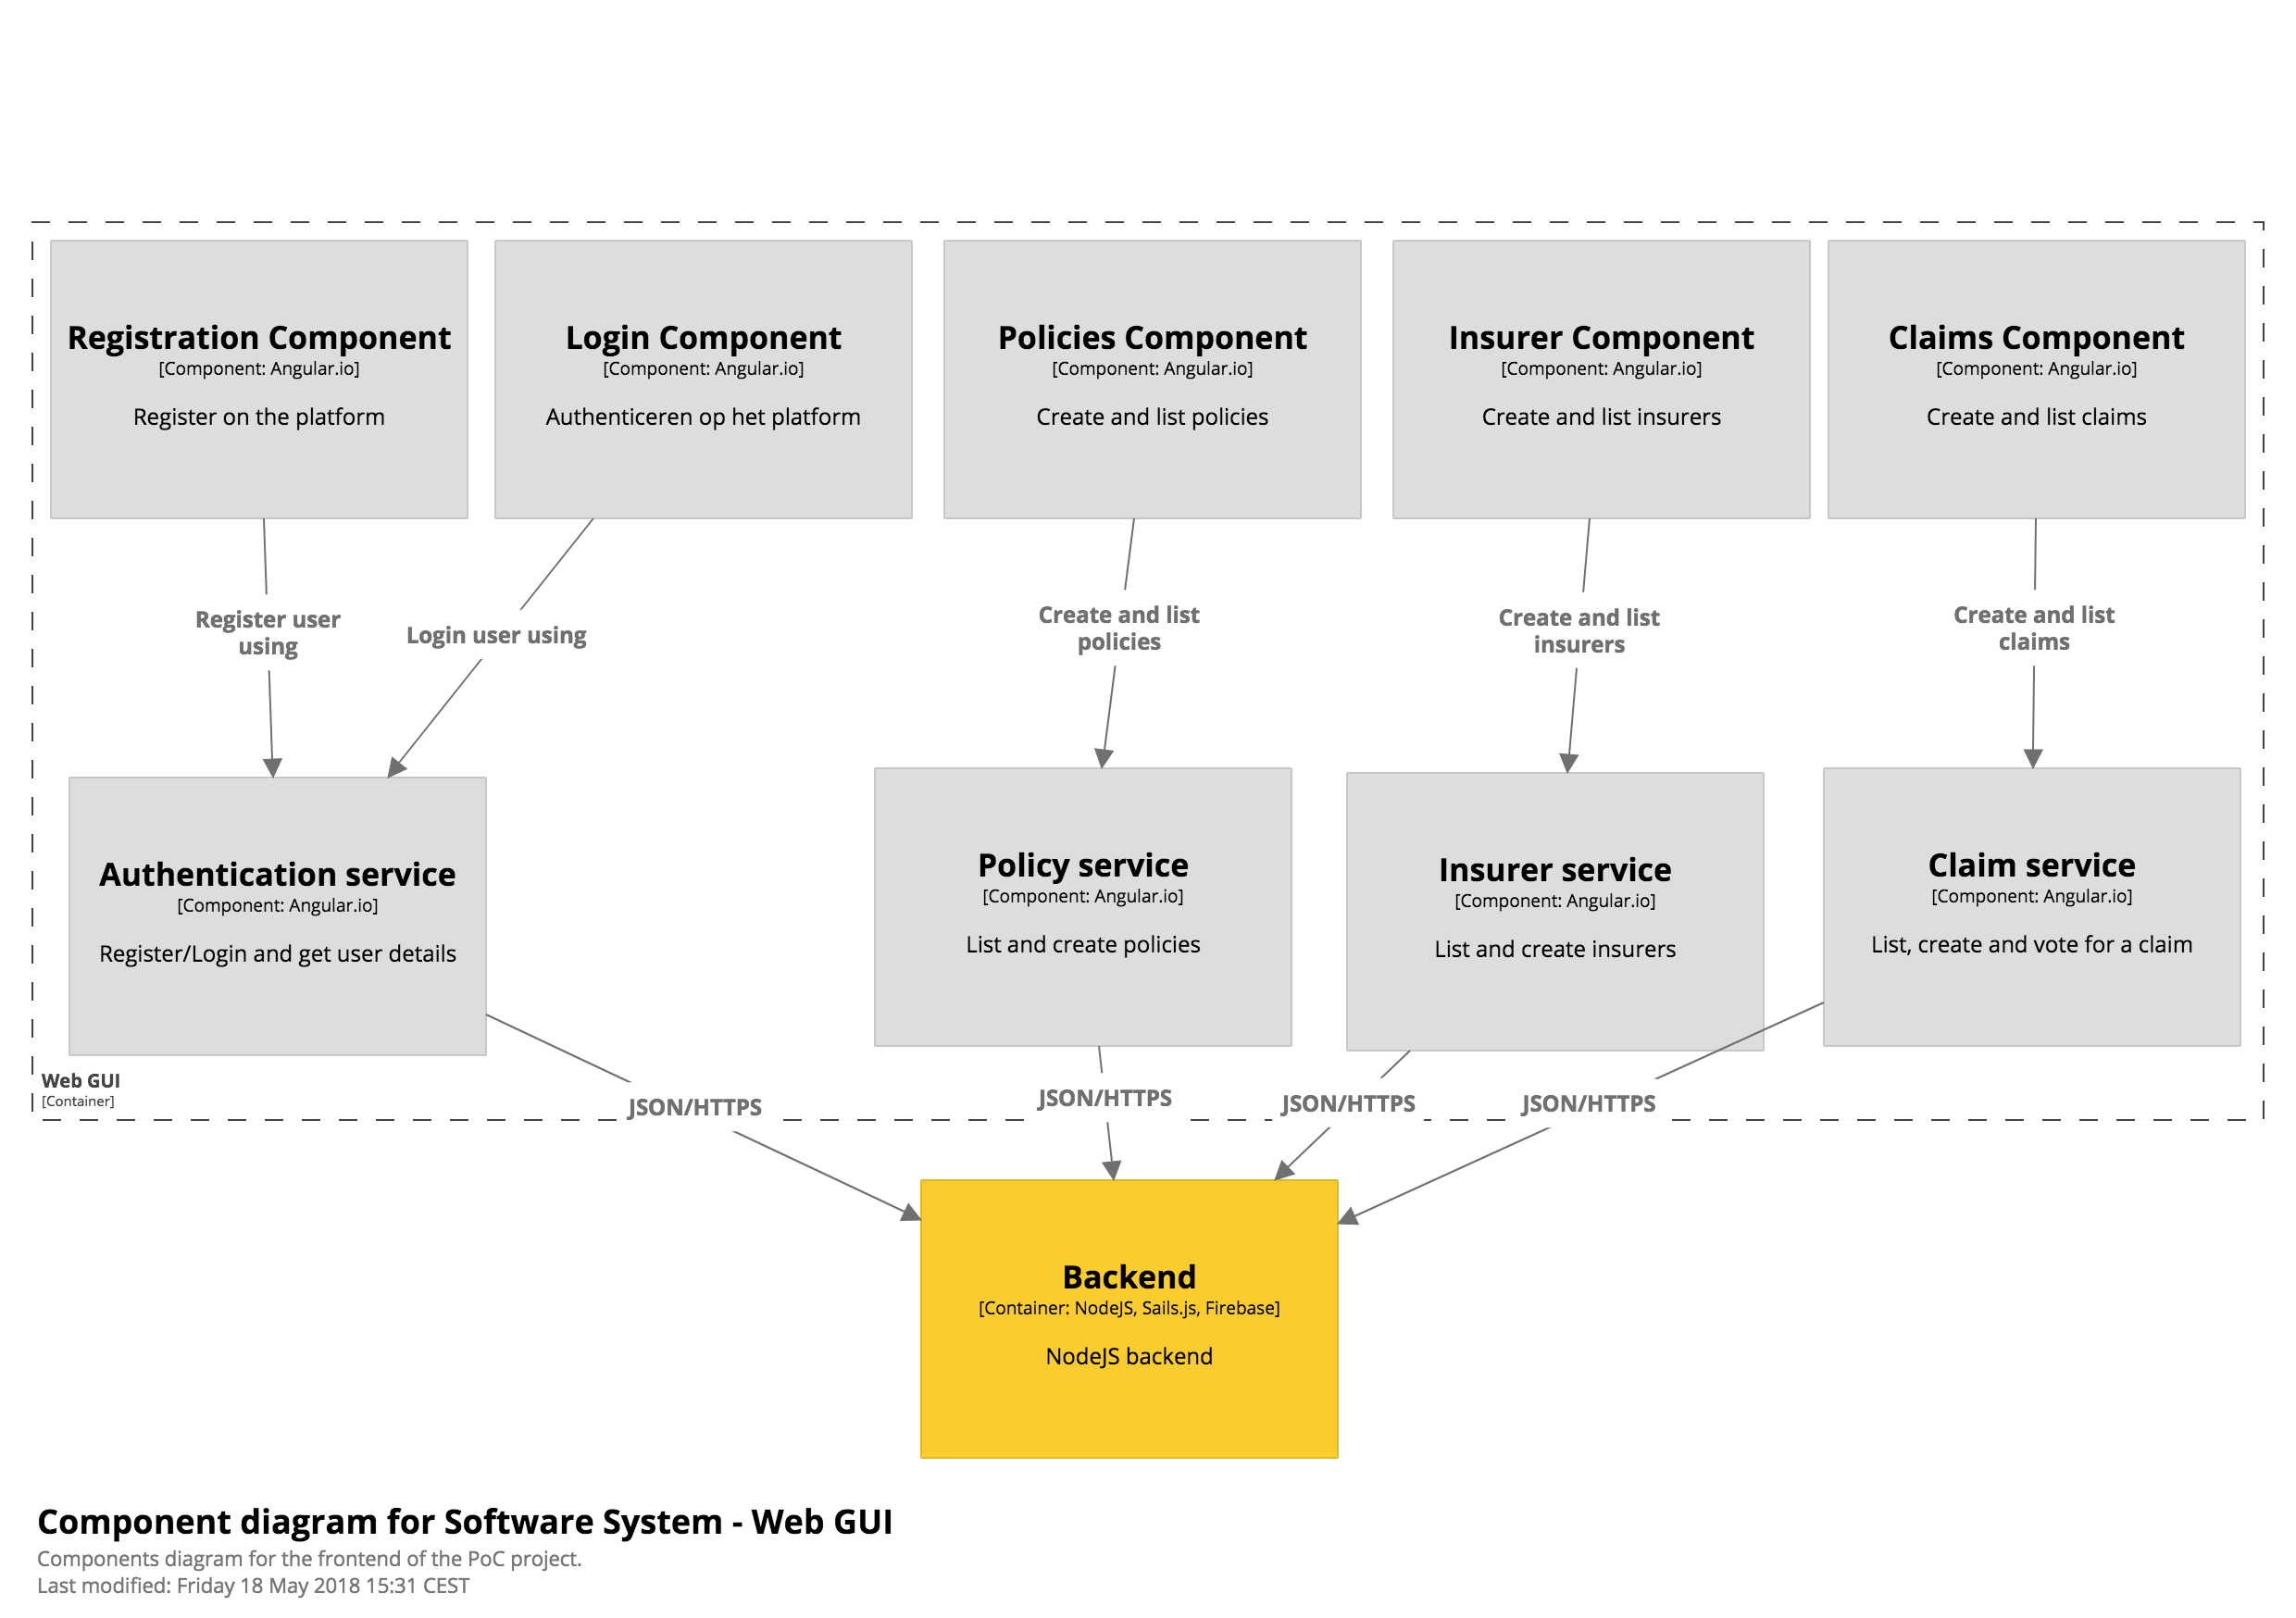
\includegraphics[width=\paperwidth-100]{images/components}
        \caption{C4 - Containers.}
        \label{fig:c4Containers}
    \end{center}
\end{figure}

In de onderstaande opsomming staan de non-functinoele requirements die ook aan het PoC worden gesteld.
\begin{itemize}
  \item \textbf{R1.} Het systeem geeft gebruikers toegang op basis van hun email en wachtwoord
  \item \textbf{R2.} Het systeem controleert bij een claim aanvraag van of het polis nummer valide is
  \item \textbf{R3.} Het systeem moet automatisch goedkeuring geven voor een claim als het claimbedrag onder 1000 euro zit en het type diefstal is.
  \item \textbf{R4.} Met gebruik van smart contracts en de blockchain wordt de data integriteit gewaarborgd.
  \item \textbf{R5.} Een verzekeraar kan bij het aanmaken van een nieuwe polis aangeven wat de verdeling is tussen de verzekeringsmaatschappijen.
\end{itemize}

The design of the final PoC was based on the requirements and user stories mentioned above.